\documentclass{standalone}
\usepackage{tikz}
\usetikzlibrary{patterns, positioning}

\begin{document}
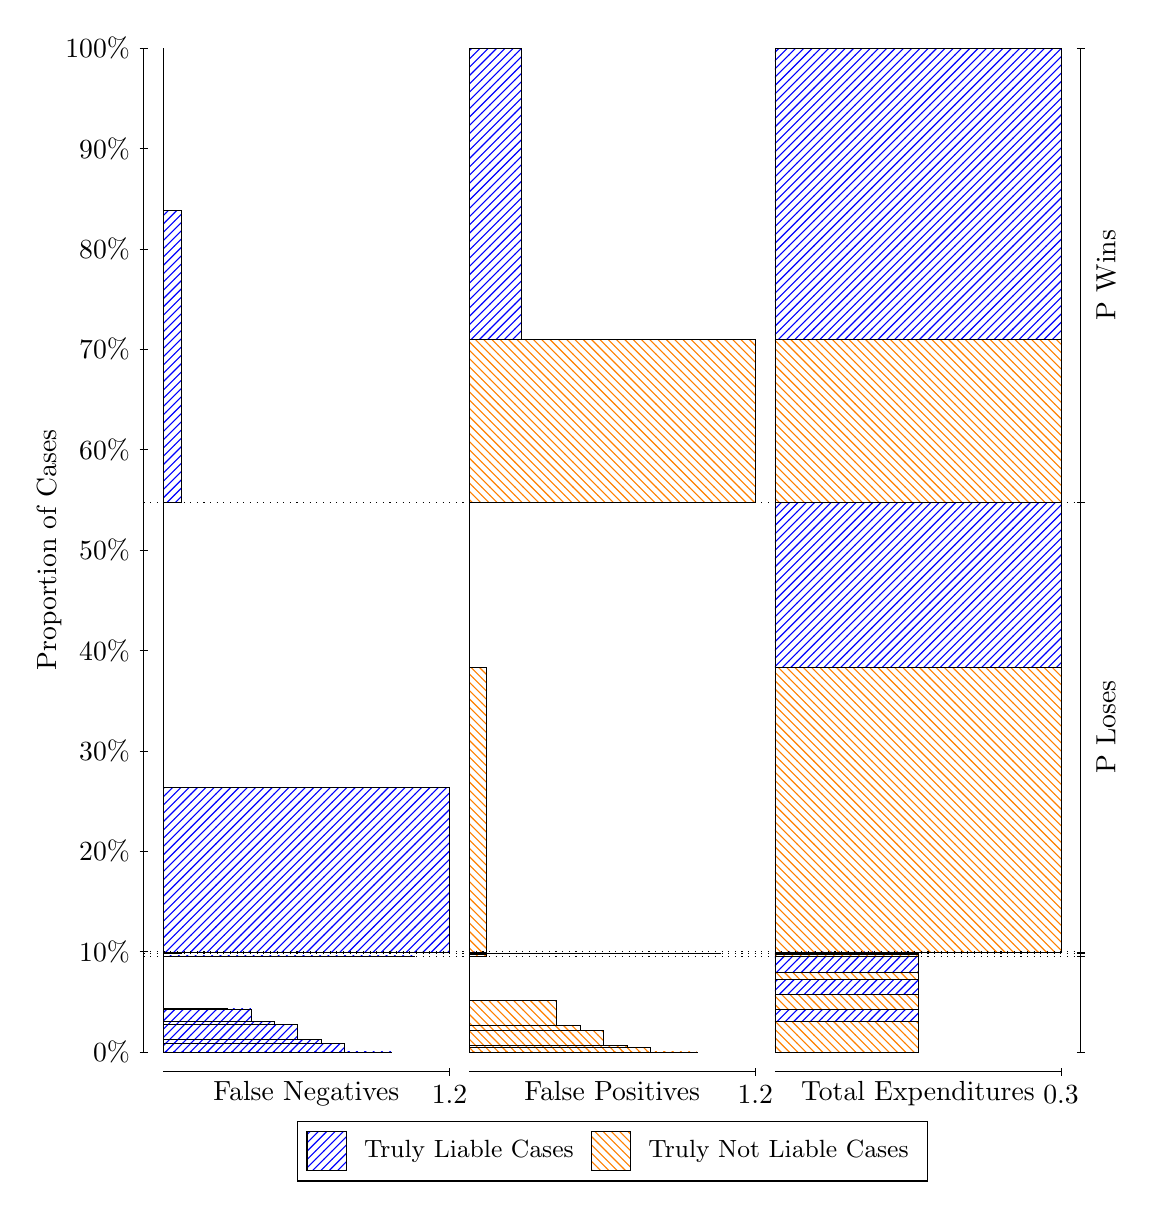
\begin{tikzpicture}
\draw[black, very thin] (1.5,1.75) -- (1.5,14.5);
\node[rotate=90, anchor=center] at (0.3, 8.125) {Proportion of Cases};
\draw[black, very thin] (1.45,1.75) -- (1.55,1.75);
\node[anchor=east] at (1.45, 1.75) {0\%};
\draw[black, very thin] (1.45,3.025) -- (1.55,3.025);
\node[anchor=east] at (1.45, 3.025) {10\%};
\draw[black, very thin] (1.45,4.3) -- (1.55,4.3);
\node[anchor=east] at (1.45, 4.3) {20\%};
\draw[black, very thin] (1.45,5.575) -- (1.55,5.575);
\node[anchor=east] at (1.45, 5.575) {30\%};
\draw[black, very thin] (1.45,6.85) -- (1.55,6.85);
\node[anchor=east] at (1.45, 6.85) {40\%};
\draw[black, very thin] (1.45,8.125) -- (1.55,8.125);
\node[anchor=east] at (1.45, 8.125) {50\%};
\draw[black, very thin] (1.45,9.4) -- (1.55,9.4);
\node[anchor=east] at (1.45, 9.4) {60\%};
\draw[black, very thin] (1.45,10.675) -- (1.55,10.675);
\node[anchor=east] at (1.45, 10.675) {70\%};
\draw[black, very thin] (1.45,11.95) -- (1.55,11.95);
\node[anchor=east] at (1.45, 11.95) {80\%};
\draw[black, very thin] (1.45,13.225) -- (1.55,13.225);
\node[anchor=east] at (1.45, 13.225) {90\%};
\draw[black, very thin] (1.45,14.5) -- (1.55,14.5);
\node[anchor=east] at (1.45, 14.5) {100\%};

\draw[black, very thin] (13.4,1.75) -- (13.4,14.5);
\draw[black, very thin] (13.35,1.75) -- (13.45,1.75);
\node[anchor=west] at (13.35, 1.75) {};
\draw[black, very thin] (13.35,2.9602) -- (13.45,2.9602);
\node[anchor=west] at (13.35, 2.9602) {};
\draw[black, very thin] (13.35,2.9973) -- (13.45,2.9973);
\node[anchor=west] at (13.35, 2.9973) {};
\draw[black, very thin] (13.35,3.0209) -- (13.45,3.0209);
\node[anchor=west] at (13.35, 3.0209) {};
\draw[black, very thin] (13.35,8.7319) -- (13.45,8.7319);
\node[anchor=west] at (13.35, 8.7319) {};
\draw[black, very thin] (13.35,14.5) -- (13.45,14.5);
\node[anchor=west] at (13.35, 14.5) {};

\draw[black, very thin, pattern color=blue, pattern=north east lines] (1.75,1.75) rectangle (4.6418,1.7507);
\draw[black, very thin, pattern color=blue, pattern=north east lines] (1.75,1.7507) rectangle (4.3452,1.7522);
\draw[black, very thin, pattern color=blue, pattern=north east lines] (1.75,1.7522) rectangle (4.0486,1.8614);
\draw[black, very thin, pattern color=blue, pattern=north east lines] (1.75,1.8614) rectangle (3.752,1.9081);
\draw[black, very thin, pattern color=blue, pattern=north east lines] (1.75,1.9081) rectangle (3.4554,2.0997);
\draw[black, very thin, pattern color=blue, pattern=north east lines] (1.75,2.0997) rectangle (3.1588,2.1369);
\draw[black, very thin, pattern color=blue, pattern=north east lines] (1.75,2.1369) rectangle (2.8622,2.298);
\draw[black, very thin, pattern color=blue, pattern=north east lines] (1.75,2.298) rectangle (2.5656,2.3004);
\draw[black, very thin, pattern color=blue, pattern=north east lines] (1.75,2.3004) rectangle (2.269,2.3024);
\draw[black, very thin, pattern color=orange, pattern=north west lines] (1.75,2.3024) rectangle (1.75,2.9602);
\draw[black, very thin, pattern color=blue, pattern=north east lines] (1.75,2.9602) rectangle (4.9384,2.9697);
\draw[black, very thin, pattern color=orange, pattern=north west lines] (1.75,2.9697) rectangle (1.75,2.9973);
\draw[black, very thin, pattern color=blue, pattern=north east lines] (1.75,2.9973) rectangle (1.9724,3.015);
\draw[black, very thin, pattern color=orange, pattern=north west lines] (1.75,3.015) rectangle (1.75,3.0209);
\draw[black, very thin, pattern color=blue, pattern=north east lines] (1.75,3.0209) rectangle (5.3833,5.1138);
\draw[black, very thin, pattern color=orange, pattern=north west lines] (1.75,5.1138) rectangle (1.75,8.7319);
\draw[black, very thin, pattern color=blue, pattern=north east lines] (1.75,8.7319) rectangle (1.9724,12.435);
\draw[black, very thin, pattern color=orange, pattern=north west lines] (1.75,12.435) rectangle (1.75,14.5);
\draw[black, very thin, pattern color=orange, pattern=north west lines] (5.6333,1.75) rectangle (8.5252,1.7506);
\draw[black, very thin, pattern color=orange, pattern=north west lines] (5.6333,1.7506) rectangle (8.2286,1.7514);
\draw[black, very thin, pattern color=orange, pattern=north west lines] (5.6333,1.7514) rectangle (7.932,1.8065);
\draw[black, very thin, pattern color=orange, pattern=north west lines] (5.6333,1.8065) rectangle (7.6354,1.8336);
\draw[black, very thin, pattern color=orange, pattern=north west lines] (5.6333,1.8336) rectangle (7.3388,2.0209);
\draw[black, very thin, pattern color=orange, pattern=north west lines] (5.6333,2.0209) rectangle (7.0422,2.0836);
\draw[black, very thin, pattern color=orange, pattern=north west lines] (5.6333,2.0836) rectangle (7.0422,2.0837);
\draw[black, very thin, pattern color=orange, pattern=north west lines] (5.6333,2.0837) rectangle (6.7456,2.4009);
\draw[black, very thin, pattern color=orange, pattern=north west lines] (5.6333,2.4009) rectangle (6.449,2.4052);
\draw[black, very thin, pattern color=orange, pattern=north west lines] (5.6333,2.4052) rectangle (6.1524,2.4078);
\draw[black, very thin, pattern color=blue, pattern=north east lines] (5.6333,2.4078) rectangle (5.6333,2.9602);
\draw[black, very thin, pattern color=orange, pattern=north west lines] (5.6333,2.9602) rectangle (5.8558,2.9879);
\draw[black, very thin, pattern color=blue, pattern=north east lines] (5.6333,2.9879) rectangle (5.6333,2.9973);
\draw[black, very thin, pattern color=orange, pattern=north west lines] (5.6333,2.9973) rectangle (8.8218,3.0033);
\draw[black, very thin, pattern color=blue, pattern=north east lines] (5.6333,3.0033) rectangle (5.8558,3.0209);
\draw[black, very thin, pattern color=orange, pattern=north west lines] (5.6333,3.0209) rectangle (5.8558,6.6391);
\draw[black, very thin, pattern color=blue, pattern=north east lines] (5.6333,6.6391) rectangle (5.6333,8.7319);
\draw[black, very thin, pattern color=orange, pattern=north west lines] (5.6333,8.7319) rectangle (9.2667,10.797);
\draw[black, very thin, pattern color=blue, pattern=north east lines] (5.6333,10.797) rectangle (6.3007,14.5);
\draw[black, very thin, pattern color=orange, pattern=north west lines] (9.5167,1.75) rectangle (11.333,2.1343);
\draw[black, very thin, pattern color=blue, pattern=north east lines] (9.5167,2.1343) rectangle (11.333,2.2916);
\draw[black, very thin, pattern color=orange, pattern=north west lines] (9.5167,2.2916) rectangle (11.333,2.4815);
\draw[black, very thin, pattern color=blue, pattern=north east lines] (9.5167,2.4815) rectangle (11.333,2.6739);
\draw[black, very thin, pattern color=orange, pattern=north west lines] (9.5167,2.6739) rectangle (11.333,2.7575);
\draw[black, very thin, pattern color=blue, pattern=north east lines] (9.5167,2.7575) rectangle (11.333,2.9602);
\draw[black, very thin, pattern color=orange, pattern=north west lines] (9.5167,2.9602) rectangle (11.333,2.9879);
\draw[black, very thin, pattern color=blue, pattern=north east lines] (9.5167,2.9879) rectangle (11.333,2.9973);
\draw[black, very thin, pattern color=orange, pattern=north west lines] (9.5167,2.9973) rectangle (11.333,3.0033);
\draw[black, very thin, pattern color=blue, pattern=north east lines] (9.5167,3.0033) rectangle (11.333,3.0209);
\draw[black, very thin, pattern color=orange, pattern=north west lines] (9.5167,3.0209) rectangle (13.15,6.6391);
\draw[black, very thin, pattern color=blue, pattern=north east lines] (9.5167,6.6391) rectangle (13.15,8.7319);
\draw[black, very thin, pattern color=orange, pattern=north west lines] (9.5167,8.7319) rectangle (13.15,10.797);
\draw[black, very thin, pattern color=blue, pattern=north east lines] (9.5167,10.797) rectangle (13.15,14.5);
\draw[black, dotted] (1.5,2.9602) -- (13.4,2.9602);
\draw[black, dotted] (1.5,2.9973) -- (13.4,2.9973);
\draw[black, dotted] (1.5,3.0209) -- (13.4,3.0209);
\draw[black, dotted] (1.5,8.7319) -- (13.4,8.7319);
\draw[black, very thin] (1.75,1.5) -- (5.3833,1.5);
\node[anchor=north] at (3.5667, 1.5) {False Negatives};
\draw[black, very thin] (5.3833,1.45) -- (5.3833,1.55);
\node[anchor=north] at (5.3833, 1.45) {1.2};

\draw[black, very thin] (5.6333,1.5) -- (9.2667,1.5);
\node[anchor=north] at (7.45, 1.5) {False Positives};
\draw[black, very thin] (9.2667,1.45) -- (9.2667,1.55);
\node[anchor=north] at (9.2667, 1.45) {1.2};

\draw[black, very thin] (9.5167,1.5) -- (13.15,1.5);
\node[anchor=north] at (11.333, 1.5) {Total Expenditures};
\draw[black, very thin] (13.15,1.45) -- (13.15,1.55);
\node[anchor=north] at (13.15, 1.45) {0.3};




\node[black, centered, rotate=90] at (13.72, 5.8764) {P Loses};
\node[black, centered, rotate=90] at (13.72, 11.616) {P Wins};

\draw (7.449999999999999,1.5) node[draw=none] (baseCoordinate) {};
\begin{scope}[align=center]
        \matrix[scale=0.5, draw=black, below=0.5cm of baseCoordinate, nodes={draw}, column sep=0.1cm]{
            \node[rectangle, draw, minimum width=0.5cm, minimum height=0.5cm, pattern=north east lines, pattern color=blue] {}; &
            \node[draw=none, font=\small] (B) {Truly Liable Cases}; &
            \node[rectangle, draw, minimum width=0.5cm, minimum height=0.5cm, pattern=north west lines, pattern color=orange] {}; &
            \node[draw=none, font=\small] (B) {Truly Not Liable Cases}; \\
            };
\end{scope}

\end{tikzpicture}
\end{document}